\documentclass[12pt, twoside]{article}
\usepackage[letterpaper, margin=1in, headsep=0.2in]{geometry}
\setlength{\headheight}{0.6in}
%\usepackage[english]{babel}
\usepackage[utf8]{inputenc}
\usepackage{microtype}
\usepackage{amsmath}
\usepackage{amssymb}
%\usepackage{amsfonts}
\usepackage{siunitx} %units in math. eg 20\milli\meter
\usepackage{yhmath} % for arcs, overparenth command
\usepackage{tikz} %graphics
\usetikzlibrary{quotes, angles}
\usepackage{graphicx} %consider setting \graphicspath{{images/}}
\usepackage{parskip} %no paragraph indent
\usepackage{enumitem}
\usepackage{multicol}
\usepackage{venndiagram}

\usepackage{fancyhdr}
\pagestyle{fancy}
\fancyhf{}
\renewcommand{\headrulewidth}{0pt} % disable the underline of the header
\raggedbottom
\hfuzz=2mm %suppresses overfull box warnings

\usepackage{hyperref}

\fancyhead[LE]{\thepage}
\fancyhead[RO]{\thepage \\ Name: \hspace{4cm} \,\\}
\fancyhead[LO]{BECA / Dr. Huson / Geometry\\*  Unit 3: Parallel lines and transversals\\* 28 October 2022}

\begin{document}

\subsubsection*{3.8 Test: Extension topics}
\emph{Diagrams are not necessarily drawn to scale unless otherwise stated.}
\begin{enumerate}
\item Given $\overline{FGHI}$, $FG=8 \frac{1}{6}$, $GH=12 \frac{1}{3}$, and $HI= 5 \frac{1}{2}$. Find the total length, ${FI}$. \par \bigskip
  \begin{tikzpicture}
    \draw[thick] (0,0)--(9,0);
    \draw[fill] (0,0) circle [radius=0.05] node[below]{$F$};
    \draw[fill] (3,0) circle [radius=0.05] node[below]{$G$};
    \draw[fill] (7,0) circle [radius=0.05] node[below]{$H$};
    \draw[fill] (9,0) circle [radius=0.05] node[below]{$I$};
  \end{tikzpicture} \vspace{2cm}

\item Given $\overleftrightarrow{JK}$ as shown on the number line. \par \smallskip
  \begin{tikzpicture}[scale=0.5]
    \draw[<->] (49,0)--(71,0);
    \foreach \x in {50, 52,...,70}
      \draw[shift={(\x,0)}] (0pt,-6pt)--(0pt,6pt) node[below=5pt]{$\x$};
    \draw[fill] (54,0) circle [radius=0.1] node[above]{$J$};
    \draw[fill] (68,0) circle [radius=0.1] node[above]{$K$};
  \end{tikzpicture} \par \smallskip
  Mark the midpoint $M$ of $J$ and $K$ on the number line with its value. \vspace{3cm}

\item The point $M(2.3)$ is the midpoint of segment $\overline{AB}$. Given $A(-1.5)$, find the value of $B$. Mark and label it below. \par \smallskip
  \begin{tikzpicture}
  \draw[<->] (-2.5,0)--(8.5,0);
  \foreach \x in {-2,...,8}
    \draw[shift={(\x,0)}] (0pt,-3pt)--(0pt,3pt) node[below=5pt]{$\x$};
  \draw[fill] (-1.5,0) circle [radius=0.05] node[above]{$A(-1.5)$};
  \draw[fill] (2.3,0) circle [radius=0.05] node[above]{$M(2.3)$};
  \end{tikzpicture} \vspace{3cm}

\item Given the rectangle $ABCD$ shown below, with $AB=6 \frac{1}{3}$ and $BC=2 \frac{1}{2}$. Find the area of the rectangle, expressing your result as a fraction.
  \begin{flushright}
  \begin{tikzpicture}[scale=1.]
    \draw[-, thick] (0,0)--(4.5,0)--(4.5,2)--(0,2)--cycle;
    \draw[fill] (0,0) circle [radius=0.05] node[left]{$A$};
    \draw[fill] (4.5,0) circle [radius=0.05] node[right]{$B$};
    \draw[fill] (4.5,2) circle [radius=0.05] node[right]{$C$};
    \draw[fill] (0,2) circle [radius=0.05] node[left]{$D$};
    \node at (5, 1){$2 \frac{1}{2}$};
    \node at (2.25, -0.5){$6 \frac{1}{3}$};
  \end{tikzpicture}
  \end{flushright}

\newpage
\item Given $\overline{PQR}$, $PQ=3x+14$, $QR=2x+5$, $PR=4x+28$. \par \smallskip
Write down an equation to represent the situation. Find $x$.
  \begin{flushleft}
    \begin{tikzpicture}
    \draw[-, thick] (0,0)--(7,0);
    \draw[fill] (0,0) circle [radius=0.05] node[below]{$P$};
    \draw[fill] (5,0) circle [radius=0.05] node[below]{$Q$};
    \draw[fill] (7,0) circle [radius=0.05] node[below]{$R$};
    \node at (2,0) [above]{$3x+14$};
    \node at (6,0) [above]{$2x+5$};
    \draw[<->, dashed] (0,-0.7)--(7,-0.7);
    \node at (3.5,-0.7) [below]{$4x+28$};
  \end{tikzpicture}
  \end{flushleft} \vspace{5cm}

\item The isosceles $\triangle FGH$ is shown with $\overline{FH} \cong \overline{GH}$. Given $GH=2x+15$ and $FH=19$. \par \smallskip
If the perimeter of the triangle is 50, find $FG$. \par \smallskip
  \begin{tikzpicture}[scale=0.5]
    \draw[thick](0,0)--(4,0)--(2,6)--(0,0);
    \draw[fill] (0,0) circle [radius=0.05] node[below left]{$F$};
    \draw[fill] (4,0) circle [radius=0.05] node[below right]{$G$};
    \draw[fill] (2,6) circle [radius=0.05] node[above right]{$H$};
    \draw[thick] (0.8,3.1)--(1.2,3); %tick mark
    \draw[thick] (2.8,3)--(3.2,3.1); %tick mark
    \node at (3.5,3.4) [right]{$2x+15$};
    \node at (0.8,3.4) [left]{$19$};
  \end{tikzpicture} \vspace{2cm}

\item Find the area of $\triangle ABC$ shown below with $m\angle C=90^\circ$ and the lengths of the triangle's sides as $a=50$, $b=87$, and $c=100$. \par \medskip
  \begin{tikzpicture}[scale=1.2]
    \draw[thick]
    (0,0)node[left]{$A$}--
    (4,0)node[below right]{$C$}--
    (4,2.31)node[right]{$B$}--cycle;
    \draw (4,0)++(-0.3,0)--++(0,0.3)--+(0.3,0);
    \node at (2,0)[below]{$b=87$};
    \node at (4,1.2)[right]{$a=50$};
    \node at (1.8,1.4)[above]{$c=100$};
  \end{tikzpicture}

\newpage
\item The protractor shown below is marked with degree measures on the inside and radian measures on the outside. Make a 1 radian angle by drawing a ray from the center $V$ through the protractor semicircle. \par \medskip
  \begin{center}
  \begin{tikzpicture}
    \draw[thick] (-3,0)--(0,0)--(3,0);
    \draw (4,0) arc (0:180:4);
    \fill (0,0) circle [radius=0.05]node[below]{$V$};
    \foreach \x in {0,15,30,...,180}
      \node at (\x:3.4){\x};
    \foreach \x in {0,15,30,...,180}
      \draw (\x:3.7)--(\x:4);
    \foreach \x in {0,5,...,180}
      \draw (\x:3.9)--(\x:4);
    \foreach \x in {0,0.1,...,3.1}
      \draw (57.3*\x:4)--(57.3*\x:4.3);
    \foreach \x in {0.2,0.4,0.6,0.8,1.0,1.2,1.4,1.6,1.8,2.0,2.2,2.4,2.6,2.8,3.0}
      \node at (57.3*\x:4.7){\x};
    \draw (-4.3,0)node[left]{$\pi$}--(-4,0);
    \draw[->,thick] (4,0)--(0:6);
    \end{tikzpicture}
  \end{center}

\item Use the protractor above to convert radians and degrees. (nearest whole degree, nearest hundredth radian).
  \begin{multicols}{2}
    \begin{enumerate}
      \item $80^\circ = $ \vspace{0.7cm}
      \item $28^\circ = $ \vspace{0.7cm}
      \item $\displaystyle 1.0 \text{ radian} =$ \vspace{0.7cm}
      \item $\displaystyle 2.7 \text{ radian} =$
    \end{enumerate}
  \end{multicols}

\item Given $x=-3$ simplify each expression. (try to do them without a calculator)
  \begin{multicols}{2}
    \begin{enumerate}[itemsep=1.25cm]
      \item $|x-1|=$
      \item $2 \times|x+2|=$
    \end{enumerate}
  \end{multicols} \vspace{1cm}

\item Find all values of $x$ satisfying the equation. (show the two cases and checks) 
  $$ |x+2|+7 = 17$$

\newpage
\item Convert each value to scientific notation.
  \begin{multicols}{2}
    \begin{enumerate}[itemsep=1cm]
      \item 70,000 =
      \item 860,000 =
    \end{enumerate}
  \end{multicols} \vspace{1cm}

\item Expand each value to regular numeric form. (i.e. an integer)
  \begin{multicols}{2}
    \begin{enumerate}[itemsep=1cm]
      \item $3 \times 10^{6}=$
      \item $1.25 \times 10^{3}=$
    \end{enumerate}
  \end{multicols} \vspace{0.7cm}

\item Round each value to the \emph{nearest hundredth}.
  \begin{multicols}{2}
    \begin{enumerate}
      \item $1 \text{ radian}=57.29577951...^\circ$ \par 
      \item $\sqrt{5} \approx$
    \end{enumerate}
  \end{multicols} \smallskip 

\item Round each value to the nearest thousand.
  \begin{multicols}{2}
    \begin{enumerate}
      \item $53,997 \approx$ \par \bigskip (the area of Florida in square miles)
      \item $42,224 \approx$ \par \bigskip (the area of New York)
    \end{enumerate}
  \end{multicols}

\item The distance in miles from New York City to Santo Domingo, Dominican Republic is 1,554 miles. Convert that distance to kilometers. Round to the \emph{nearest whole kilometer}. (1 mile $\approx$ 1.61 kilometers) \vspace{2cm}

\emph{Use the formula for percent error in the following problem}
$$\epsilon = \left|\frac{v_A-v_E}{v_E}\right| \times 100\%$$

\item The actual length of earth's year is about 365.25 days. Find the percent error of using an approximation of 360 days. Round to three significant figures.

\item Mark the positions of the minute and hour hands at 4:00. Write down the measure in degrees of the angle made by the two clock hands. \par \vspace{0.25cm}
  \begin{tikzpicture}
    \draw (0,0) circle [radius=2];
    \draw (0,0) circle [radius=0.1];
    \foreach \x in {1,...,12}
      \node at ({90+\x*-30}:1.8){\x};
  \end{tikzpicture}

\item A compound shape composed of two rectangles is shown with dimensions marked, both having heights of 6 cm and with base lengths of 2 cm and 5 cm respectively.
  \begin{multicols}{2}
    \begin{tikzpicture}
      \draw[thick] (0,0) rectangle (6,5);
      \draw[thick] (2,0) -- (2,5);
      \node at (6.5,3){6};
      \node at (1,-0.4){2};
      \node at (4,-0.4){5};
    \end{tikzpicture}
    \begin{enumerate}
      \item Find the perimeter of the smaller rectangle on the left. \vspace{2cm}
      \item Find the total area of the combined rectangles
      \end{enumerate}
    \end{multicols} \vspace{1cm}

\end{enumerate}
\end{document}